\section{第四章}



\subsection{题目1}

以$y=sin(x)$为例,在$[0,\pi]$区间内生成11个、21个数据点,设计算法或程序,用上述四个边界条件(自然边界、固定边界、周期边界、强制第一个子区间和第二个子区间样条多项式的三阶导数相等,倒数第二个子区间和最后一个子区间的三次样条函数的三阶导数相等),分别计算其样条插值,并作图比较,分析其差异性。

\paragraph{样条插值}

顾名思义,分段就是把区间$[a,b]$分成n个区间,共有n+1个点,其中两个端点$x_0=a,x_n=b$。三次样条就是说每个小区间的曲线是一个三次方程,三次样条方程满足以下条件:

1,在每个分段小区间$[x_i,x_{i+1}]$上, $S(x)=S_i(x)$都是一个三次方程

2,满足插值条件,即$S(x_i)=y_i \quad (i=0,1,\cdots ,n)$

3, 曲线光滑,即 $S(x),S'(x),S''(x)$ 连续

则这个三次方程可以构造成如下形式:

$y=a_i+b_i x+c_i x^2+d_i x^3$ 这种形式,我们称这个方程为三次样条函数 $S_i(x)$ 。

从 $S_i(x)$ 可以看出每个小区间有四个未知数 $(a_i,b_i,c_i,d_i)$ ,有n个小区间,则有4n个未知数,要解出这些未知数,则我们需要4n个方程来求解。

\paragraph{自然边界(Natural Spline)}

指定端点二阶导数为0,$S''(x_0)=0=S''(x_n)$


\paragraph{固定边界(Clamped Spline)}

指定端点一阶导数,这里分别为A和B,即$S'_0=A, S'_{n-1}(x_n)=B$

\paragraph{非扭结边界(Not-A-Knot Spline)}

强制第一个插值点的三阶导数值等于第二个点的三阶导数值,最后第一个点的三阶导数值等于倒数第二个点的三阶导数值. 即$S'''_0(x_0)=S'''_1(x_1) \quad and \quad S'''_{n-2}(x_{n-1})=S'''_{n-1}(x_n)$

\paragraph{周期边界(Periodic Spline)}

要求样条S(x)及其导函数是以区间长度$x_n-x_0$为周期的函数,即$S(x_0)=S(x_n),S'(x_0)=S'(x_n),S''(x_0)=S''(x_n)$

\paragraph{绘图}

分别将$[0,\pi]$等分成11段与21段,带入写好的样条插值函数中,计算对应的样条插值。然后,在$[0,\pi]$区间内,均匀的去50个点并将其映射到坐标轴上,得到如下两图:


\begin{figure}[H]
\centering
\begin{minipage}[t]{0.48\textwidth}
\centering
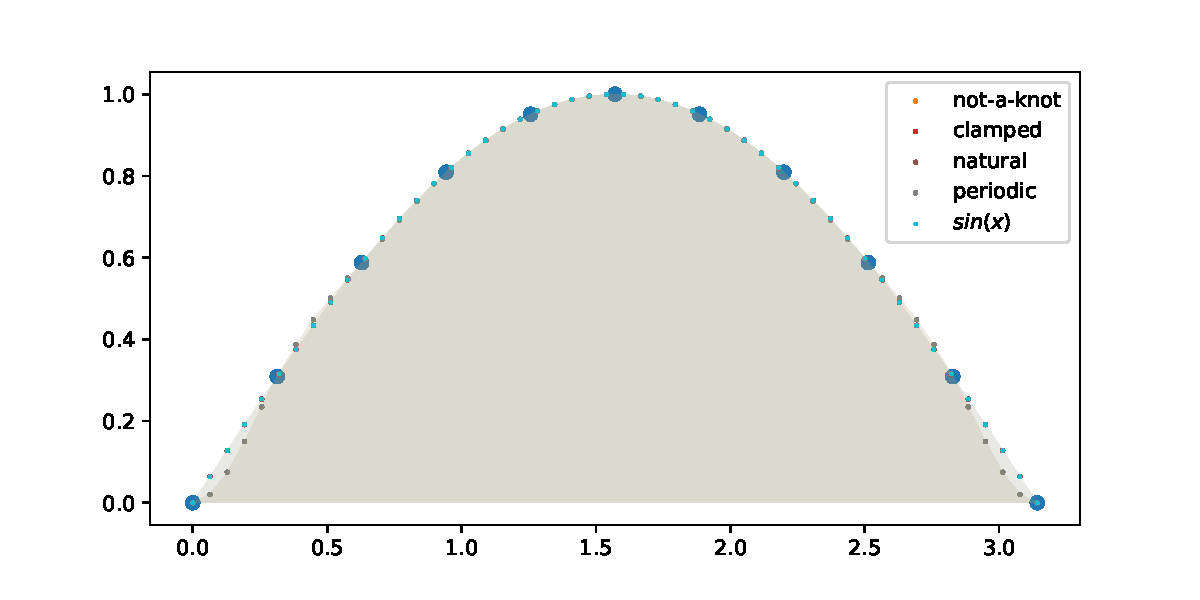
\includegraphics[width=6cm]{4-1.pdf}
\caption{$[0,\pi]$等分11段插值结果}
\end{minipage}
\begin{minipage}[t]{0.48\textwidth}
\centering
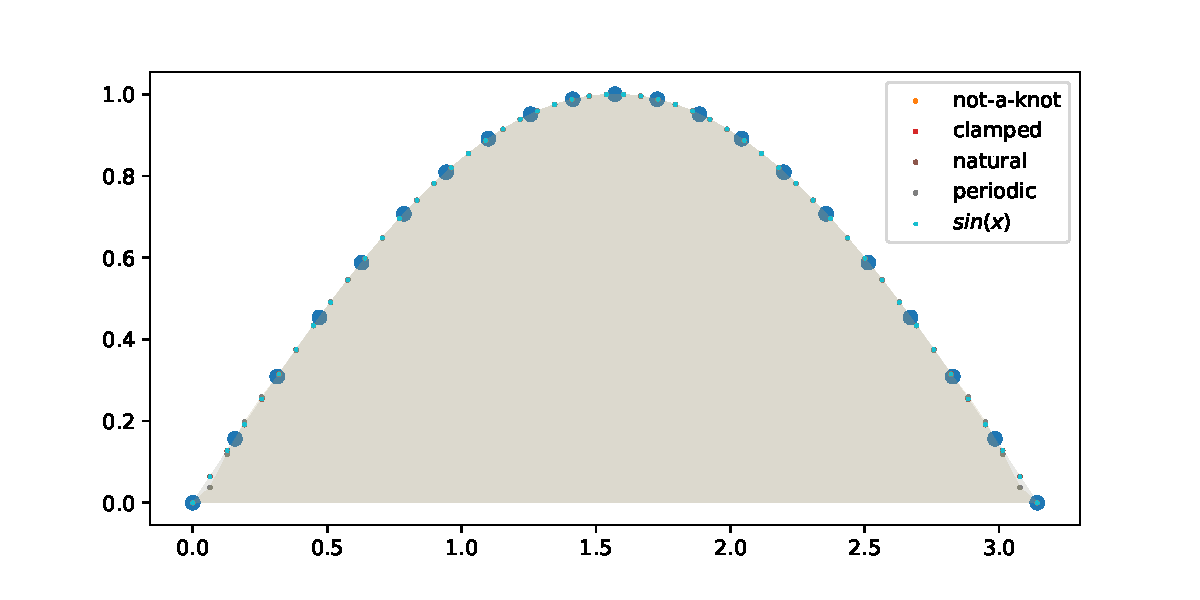
\includegraphics[width=6cm]{4-3.pdf}
\caption{$[0,\pi]$等分21段插值结果}
\end{minipage}
\end{figure}

可以观察到,由于三次拟合的情况较为良好,很难观察出不同节点之间的拟合情况,于是通过选择不同的映射点的个数,绘制下图

\begin{figure}[H]
	\centering
	\caption{不同边界条件插值绘制结果}
	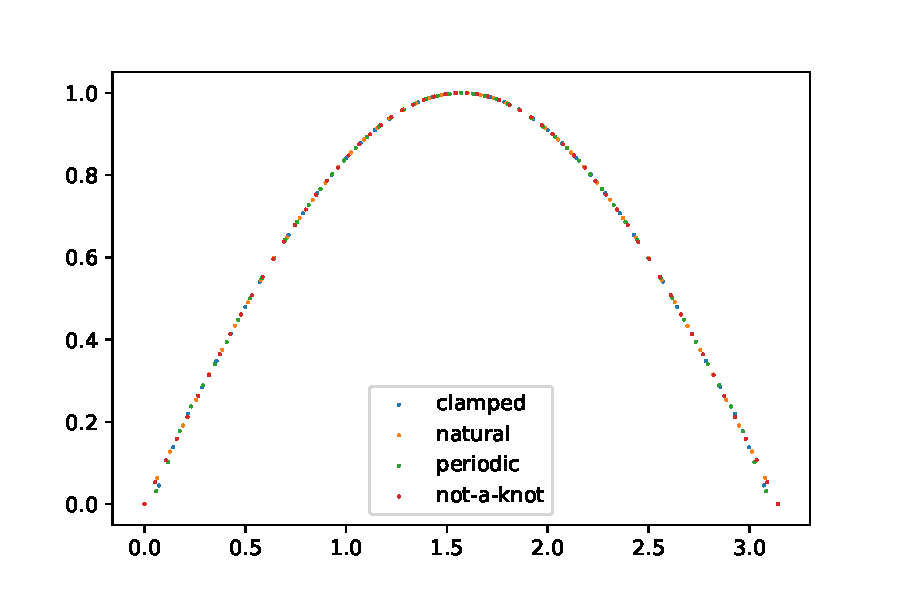
\includegraphics[width=.9\linewidth]{4-4.pdf}
\end{figure}

\paragraph{计算结果展示}


为了更好地展示所计算样条插值的结果,我们选取了插值计算后的前十个点,进行展示。下图是$[0,\pi]$区间内,选取50个点,前十个点经过sin(x)函数和不同边界条件的样条插值函数的计算结果


\begin{table}[H]
	\centering
	\caption{不同边界条件的样条插值函数的计算结果}
	\begin{tabular}{lllll}
		\hline
		sin         & clamped     & natural     & periodic    & not-a-knot  \\ \hline
		0           & 0           & 0           & 0           & 0           \\
		0.058144829 & 0.017166528 & 0.058141909 & 0.017166528 & 0.058212405 \\
		0.116092914 & 0.062694079 & 0.116088532 & 0.062694079 & 0.116180395 \\
		0.173648178 & 0.1276246   & 0.173644584 & 0.1276246   & 0.17372376  \\
		0.230615871 & 0.203000041 & 0.230614781 & 0.203000041 & 0.230662291 \\
		0.286803233 & 0.279862351 & 0.286803836 & 0.279862351 & 0.286815778 \\
		0.342020143 & 0.34965416  & 0.342017152 & 0.34965416  & 0.342004013 \\
		0.396079766 & 0.409813501 & 0.39607043  & 0.409813501 & 0.396046786 \\
		0.44879918  & 0.462393675 & 0.448787296 & 0.462393675 & 0.448763886 \\
		0.5         & 0.509566705 & 0.49999158  & 0.509566705 & 0.499975106 \\ \hline

	\end{tabular}
\end{table}



\paragraph{三次样条插值代码}


\begin{minted}{python}
def calculateEquationParameters(x):
    # parameter为二维数组,用来存放参数,sizeOfInterval是用来存放区间的个数
    parameter = []
    sizeOfInterval = len(x)-1
    i = 1
    # 首先输入方程两边相邻节点处函数值相等的方程为2n-2个方程
    while i < len(x)-1:
        data = init(sizeOfInterval*4)
        data[(i-1)*4] = x[i]*x[i]*x[i]
        data[(i-1)*4+1] = x[i]*x[i]
        data[(i-1)*4+2] = x[i]
        data[(i-1)*4+3] = 1
        data1 = init(sizeOfInterval*4)
        data1[i*4] = x[i]*x[i]*x[i]
        data1[i*4+1] = x[i]*x[i]
        data1[i*4+2] = x[i]
        data1[i*4+3] = 1
        temp = data[2:]
        parameter.append(temp)
        temp = data1[2:]
        parameter.append(temp)
        i += 1
   # 输入端点处的函数值。为两个方程, 加上前面的2n - 2个方程,一共2n个方程
    data = init(sizeOfInterval * 4 - 2)
    data[0] = x[0]
    data[1] = 1
    parameter.append(data)
    data = init(sizeOfInterval * 4)
    data[(sizeOfInterval - 1) * 4] = x[-1] * x[-1] * x[-1]
    data[(sizeOfInterval - 1) * 4 + 1] = x[-1] * x[-1]
    data[(sizeOfInterval - 1) * 4 + 2] = x[-1]
    data[(sizeOfInterval - 1) * 4 + 3] = 1
    temp = data[2:]
    parameter.append(temp)
    # 端点函数一阶导数值相等为n-1个方程。加上前面的方程为3n-1个方程。
    i = 1
    while i < sizeOfInterval:
        data = init(sizeOfInterval * 4)
        data[(i - 1) * 4] = 3 * x[i] * x[i]
        data[(i - 1) * 4 + 1] = 2 * x[i]
        data[(i - 1) * 4 + 2] = 1
        data[i * 4] = -3 * x[i] * x[i]
        data[i * 4 + 1] = -2 * x[i]
        data[i * 4 + 2] = -1
        temp = data[2:]
        parameter.append(temp)
        i += 1
    # 端点函数二阶导数值相等为n-1个方程。加上前面的方程为4n-2个方程。
    且端点处的函数值的二阶导数为零,为两个方程。总共为4n个方程。
    i = 1
    while i < len(x) - 1:
        data = init(sizeOfInterval * 4)
        data[(i - 1) * 4] = 6 * x[i]
        data[(i - 1) * 4 + 1] = 2
        data[i * 4] = -6 * x[i]
        data[i * 4 + 1] = -2
        temp = data[2:]
        parameter.append(temp)
        i += 1
    return parameter


"""
对一个size大小的元组初始化为0
"""


def init(size):
    j = 0
    data = []
    while j < size:
        data.append(0)
        j += 1
    return data


"""
功能:计算样条函数的系数。
参数:parametes为方程的系数,y为要插值函数的因变量。
返回值:三次插值函数的系数。
"""


def solutionOfEquation(parametes, y):
    sizeOfInterval = len(x) - 1
    result = init(sizeOfInterval*4-2)
    i = 1
    while i < sizeOfInterval:
        result[(i-1)*2] = y[i]
        result[(i-1)*2+1] = y[i]
        i += 1
    result[(sizeOfInterval-1)*2] = y[0]
    result[(sizeOfInterval-1)*2+1] = y[-1]
    a = np.array(calculateEquationParameters(x))
    b = np.array(result)
    for data_x in b:
        print(data_x)
    return np.linalg.solve(a, b)


"""
功能:根据所给参数,计算三次函数的函数值:
参数:parameters为二次函数的系数,x为自变量
返回值:为函数的因变量
"""


def calculate(paremeters, x):
    result = []
    for data_x in x:
        result.append(paremeters[0]*data_x*data_x*data_x+paremeters[1]
                      * data_x*data_x+paremeters[2]*data_x+paremeters[3])
    return result


"""
功能:将函数绘制成图像
参数:data_x,data_y为离散的点.new_data_x,
new_data_y为由拉格朗日插值函数计算的值。x为函数的预测值。
返回值:空
"""


def Draw(data_x, data_y, new_data_x, new_data_y):
    plt.plot(new_data_x, new_data_y, label="拟合曲线", color="black")
    plt.scatter(data_x, data_y, label="离散数据", color="red")
    mpl.rcParams['font.sans-serif'] = ['SimHei']
    mpl.rcParams['axes.unicode_minus'] = False
    plt.title("三次样条函数")
    plt.legend(loc="upper left")
    plt.show()
\end{minted}









\pagebreak